\documentclass[12pt,a4paper]{article}   % 12pt + A4 required by the assignment
\usepackage{graphicx} % Required for inserting images

% ---- formatting required by the assignment: Times New Roman, 12pt, spacing 1.15 ----
% Applies everywhere, including tables and captions (no smaller fonts, no scaled tables).
\usepackage[T1]{fontenc}
\usepackage[utf8]{inputenc}
\usepackage{newtxtext,newtxmath}
\usepackage[top=1.8cm,bottom=1.8cm,left=2cm,right=2cm]{geometry}
\usepackage{setspace}
\setstretch{1.15}

% ---- tables, figures, captions ----
\usepackage{booktabs}
\usepackage{float}
\usepackage{array}
\usepackage[labelfont=bf,skip=3pt]{caption}   % captions in 12pt like the text
\usepackage[compact]{titlesec}
\usepackage{url}
\usepackage[hidelinks]{hyperref}

% ---- compact headings so each task fits on one page ----
\titleformat{\section}{\large\bfseries}{\thesection}{0.6em}{}
\titleformat{\subsection}{\normalsize\bfseries}{\thesubsection}{0.5em}{}
\titlespacing*{\section}{0pt}{0pt}{3pt}
\titlespacing*{\subsection}{0pt}{2pt}{0pt}
\setlength{\parindent}{0pt}
\setlength{\parskip}{3pt}
\setlength{\tabcolsep}{4pt}
\setlength{\textfloatsep}{6pt}
\setlength{\floatsep}{4pt}
\setlength{\intextsep}{4pt}

\newcommand{\ra}{$\rightarrow$}

\title{RecSys Group Project\\[4pt]
  \large DSAIT4335 Recommender Systems -- Final Project Report\\[2pt]
  \large Group 26}
\author{
  Andrei Ionita \and Vlad Alexan \and Traian Dobrin \and Rick van Loon \and Mihai-Radu Serban\\[6pt]
}
\date{\today}

\begin{document}

% First page: group information and a short introduction
\maketitle
\thispagestyle{empty}
\pagestyle{empty}

\vspace{1cm}
This report presents our work on the final project of DSAIT4335. On MovieLens-100K, we built eleven individual recommenders and four hybrids, evaluated them on both accuracy and beyond-accuracy metrics, and applied four reranking methods aimed at diversity, calibration and fairness. Each task has its own section, in which we explain the choices we made and what the results told us, with additional tables and figures being collected in the appendix. A theme that recurs throughout is the strong role of popularity in this dataset, which shapes both how our models behave and what the rerankers are able to change.

\newpage

%% =====================================================================
\section{Task 1: Building the recommenders}
%% =====================================================================

\subsection{Task 1.1 -- Selecting the individual models}

We use MovieLens-100K: 100,000 ratings from 943 users on
1,682 films. Every rating is treated as an implicit positive,
including low ratings. The nominal 80/10/10 user-grouped
random split (seed 2020) produces 80,808 training, 9,596
validation and 9,596 test interactions.

We configure eleven individual recommenders from the course
RecBole fork (Table~\ref{tab:rationale}), grouping related
models to examine contrasting design choices.
ItemKNN and UserKNN compute similarity between films or
between users. SLIM learns sparse nonnegative item--item
weights iteratively, whereas EASE computes dense weights
in closed form. Both avoid negative sampling; the small
catalogue makes EASE computationally practical.
BPR learns a free user vector with a pairwise ranking loss,
whereas FISM constructs user representations from interacted
items and, in this implementation, uses pointwise binary
cross-entropy. This examines free parameters versus
history-derived representations without assuming either
better serves users with few interactions. NeuMF combines
a multiplicative factor branch with an MLP branch and uses
pointwise binary cross-entropy, so its comparison with BPR
also involves different training objectives. NGCF and
LightGCN propagate information over the user--item graph;
LightGCN removes feature transformations and nonlinear
activations. Random and Pop provide non-personalised
references, with Pop testing how much interaction recovery
can be explained by training popularity alone.

\begin{table}[H]
\centering
\begin{tabular}{@{}p{0.2\linewidth}p{0.8\linewidth}@{}}
\toprule
Models & Rationale and relevant limitation \\
\midrule
Random & Non-personalised reference for chance-level relevance and broad exposure. \\
Pop & Global popularity ordering, filtered by user history. Tests popularity's explanatory power. \\
ItemKNN, UserKNN & Item- versus user-neighbourhood similarity. Transparent local collaborative signals, limited by sparse support. \\
SLIM, EASE & Sparse nonnegative versus dense closed-form item--item weights. Suitable candidates for a small catalogue, but catalogue size limits scalability. \\
BPR, FISM$^*$ & Free user factors versus history-derived item-factor profiles. Pairwise BPR loss versus pointwise binary cross-entropy in this FISM implementation. \\
NeuMF & Combines multiplicative-factor and MLP branches. Tests a more flexible interaction function with greater estimation demands. \\
NGCF$^*$, LightGCN & Graph propagation with versus without feature transformations and nonlinear activations. Tests multi-hop collaborative signals. \\
\bottomrule
\end{tabular}
\caption{Individual-model selection. SLIM denotes SLIMElastic; $^*$supplementary models.}
\label{tab:rationale}
\end{table}

\paragraph{Discussion.}
The full interaction matrix has 6.3\% density (5.1\% for training), yet support remains uneven: the most popular 20\% of films receive 65.0\% of training interactions. This motivates strong popularity and neighbourhood references alongside learned item--item models. Latent-factor, neural and graph approaches test whether more expressive or shared representations add complementary information. CPU constraints motivated representative families rather than an exhaustive architecture catalogue. Sequential models were outside our random-split design; other untested methods are not presumed inferior. Metadata enters through FeatureCombination in Task~1.4. Treating every rating as positive measures interaction recovery rather than explicit liking, and random splitting does not establish performance under temporal change.

\clearpage
\subsection{Task 1.2 -- Tuning the individual models}

We select configurations and checkpoints by validation MRR@10, prioritising the first relevant result. Test scores do not select settings. The search contains \textbf{61 individual-model configurations}: 49 primary configurations, including fixed Random/Pop references, and 12 supplementary configurations. Selected joint candidates cover neighbourhood sizes 25--200, embedding dimensions 32--128, learning rates 0.001--0.005 and model-specific regularisation; these ranges are not a full Cartesian grid. Exact candidates are recorded in \texttt{task1/search\_spaces.yaml}.

Trainable embedding/neural/graph models use Adam, at most 20 epochs, per-epoch validation and patience 10. Batch size is 2,048, except LightGCN (4,096). NeuMF trains both branches from scratch. Primary-model settings are fixed after seed-2020 selection and repeated on seeds 2021/2022; both splitting and stochastic training change. FISM and NGCF are evaluated on seed 2020 only.

\begin{table}[H]
\centering
\begingroup
\setlength{\tabcolsep}{3pt}
\begin{tabular}{@{}l>{\raggedright\arraybackslash}p{0.39\linewidth}rr@{}}
\toprule
Model ($n$) & Selected settings & Val MRR & Test nDCG \\
\midrule
Random (1) & Fixed random reference & .0117 & $.0080\pm.0004$ \\
Pop (1) & Training interaction counts & .1846 & $.1060\pm.0225$ \\
ItemKNN (5) & $k=75$ & .3795 & $.2762\pm.0056$ \\
UserKNN (5) & $k=50$ & .4010 & $.2819\pm.0124$ \\
BPR (8) & $d=64$, $\eta=.003$, $r=10^{-5}$ & .3777 & $.2772\pm.0104$ \\
FISM (6) & $d=64$, $\alpha=0$, $\eta=.001$; \newline $r_1=r_2=.001$ & .3313 & $.2427^*$ \\
SLIM (8) & $\alpha=.2$, L1 ratio $=.01$ & .4225 & $.3283\pm.0082$ \\
EASE (5) & $r=350$ & .4202 & $.3268\pm.0080$ \\
NeuMF (8) & $d_{\rm MF}=d_{\rm MLP}=64$, MLP [128,64], dropout .1, $\eta=.001$ & .3701 & $.2753\pm.0093$ \\
NGCF (6) & $d=64$, layers [64,64], node/message dropout $0/.1$, $\eta=.001$, $r=10^{-5}$ & .3045 & $.2104^*$ \\
LightGCN (8) & $d=64$, 2 layers, $\eta=.005$, $r=10^{-5}$ & .3428 & $.2509\pm.0107$ \\
\bottomrule
\end{tabular}
\endgroup
\caption{Counts $n$, selected settings, seed-2020 validation MRR@10 and test nDCG@10 (three-seed mean $\pm$ sample SD; $^*$one seed). $d$: embedding size; $\eta$: learning rate; $r$: model-specific regularisation.}
\label{tab:search}
\label{tab:task1}
\end{table}

\paragraph{Discussion.}
Validation evidence supports tuning rather than assuming defaults suffice. For BPR with $d=64$ and $r=10^{-5}$, MRR rises from .3474 at learning rate .001 to .3777 at .003, then falls slightly to .3750 at .005. EASE performs similarly at regularisation 250/350/500 (.4201/.4202/.4189), but worse at 50 (.3959). These observations support an intermediate learning rate and a broad regularisation plateau, not a universal optimum. SLIM and EASE lead the observed individual-model test means; their advantage is consistent with useful item co-occurrence signals, but architecture, losses and training budgets are not controlled independently. BPR, FISM and LightGCN achieve their best saved validation score at the final allowed epoch, so convergence is unestablished. Three splits describe sensitivity to splitting and training randomness; their standard deviations do not establish statistical significance or model equivalence.

\clearpage
\subsection{Task 1.3 -- Regression-weighted hybrid}

WeightedHybrid freezes all eleven individual models and learns a linear blend. The intended complementarity is between local neighbourhoods, learned item--item relations and latent/graph representations. Because their score scales differ, each model's scores are min--max normalised separately per user over nonpadding items unseen in training. Constant ranges become zero. This score scaling uses no test labels.

Regression examples comprise all 9,596 validation positives and five uniformly sampled unobserved items per positive (47,980 negatives). Sampling is without replacement per user and excludes training and validation positives. We solve constrained least squares using SLSQP:
\[
\min_{b,\mathbf{w}}\frac{1}{N}\sum_{n=1}^{N}
\left(b+\mathbf{x}_{n}^{\top}\mathbf{w}-y_n\right)^2,
\qquad w_m\geq0,\quad\sum_m w_m=1.
\]
Here $\mathbf{x}_n$ contains normalised component scores and $y_n\in\{0,1\}$. Nonnegative sum-to-one weights provide a convex blend; correlated components may still have unstable or interchangeable coefficients. The intercept is fitted but is constant across a user's items, so it does not affect ranking. Validation results are fitting diagnostics, not independent generalisation estimates. Test evaluation masks training and validation history.

\begin{table}[H]
\centering
\begin{tabular}{lr@{\hspace{1.5em}}lr}
\toprule
Component & Weight & Component & Weight \\
\midrule
SLIM & .3535 & UserKNN, BPR & $\approx0$ \\
NeuMF & .3524 & FISM, NGCF, LightGCN & $\approx0$ \\
EASE & .2494 & Pop, Random & $\approx0$ \\
ItemKNN & .0447 & & \\
\bottomrule
\end{tabular}
\caption{Reference WeightedHybrid coefficients, fitted on all validation users (seed 2020; negative ratio 5). Test MRR@10 is .5336 and nDCG@10 is .3343, versus .5310/.3308 for EASE. Values near zero include numerical solver tolerances.}
\label{tab:wh}
\end{table}

\paragraph{Discussion.}
Four components receive appreciable weight, while seven receive effectively none. BPR and UserKNN remain useful standalone models despite negligible hybrid coefficients: coefficient allocation measures their role under this regression objective and component set, not general recommendation quality. The retained models combine learned item--item relations with a neural factor/MLP score, but weights alone do not establish complementarity. The nDCG improvement over EASE is modest (.0035 on this split). Tasks 2.3--2.4 examine list overlap and component removal to distinguish redundancy from useful contributions. Coefficients are not shares of achieved accuracy or actual top-list score contribution. Finally, unobserved negatives are assumed rather than verified dislikes and can include future test positives; test labels are deliberately not inspected during sampling.

\clearpage
\subsection{Task 1.4 -- Feature-combination and switching hybrids}

We implement two further designs to test different forms of complementarity. \emph{FeatureCombination} integrates metadata with learned collaborative features. Its inputs concatenate 32-dimensional user/item embeddings, their elementwise product, binary item genres, user genre profiles, item/user text vectors and normalised log training popularity. Text uses title plus description, English-stopword TF-IDF (at most 5,000 terms), a 32-dimensional SVD projection and row normalisation. User metadata profiles average training-history item features. The text transform uses available catalogue metadata, including held-out items, but no held-out interaction labels.

A ReLU hidden layer and scalar output predict relevance. Training minimises mean $\log(1+\exp(s_{u,j}-s_{u,i}))$ for positive $i$ and uniformly sampled negative $j$, plus squared-parameter regularisation. \emph{SwitchingHybrid} instead selects either FeatureCombination's or SLIM's entire score row using the user's training activity. This tests whether metadata and collaborative models serve different history lengths; both still require training history. Validation selection allows either single-model endpoint to win (Task~1.5).

\begin{table}[H]
\centering
\begin{tabular}{lrr}
\toprule
FeatureCombination variant & Test nDCG@10 & Coverage@10 \\
\midrule
Full model & .2482 & .2170 \\
Without text & .2448 & .1950 \\
Without genres & .2344 & .1671 \\
Without popularity & .1295 & .0375 \\
Interaction features only & .1321 & .0392 \\
\bottomrule
\end{tabular}
\caption{Seed-2020 feature ablations, retrained with the full model's selected hyperparameters and training budget, without separate retuning. Interaction-only disables genres, text and popularity while retaining the embedding/product network.}
\label{tab:fc}
\end{table}

\paragraph{Discussion.}
The full feature model improves substantially over its interaction-only variant, but remains below EASE and SLIM. Removing popularity causes the largest drop; among content features, removing genres hurts accuracy more than removing text. Text removal also reduces coverage from .2170 to .1950. These are conditional findings under fixed hyperparameters: they neither prove optimal feature importance nor establish cold-item recovery. Learned user embeddings and history-derived profiles prevent interpreting this model as a history-free cold-start solution. Switching is operational, but none of the eight tested nonconstant rules exceeds SLIM's validation MRR; selection retains the SLIM-only endpoint. This is a negative result about the tested activity thresholds, not proof that metadata cannot help any user group. These designs were prioritised to examine feature interaction and user-dependent selection within the available budget.

\clearpage
\subsection{Task 1.5 -- Tuning the hybrids}

FeatureCombination has eight candidates: hidden size $\{64,128\}$, learning rate $\{.001,.003\}$ and regularisation $\{10^{-5},10^{-4}\}$. The winner uses 64 hidden units, learning rate .003 and regularisation $10^{-4}$ (validation MRR .3707). Training uses Adam, batch size 2,048, at most 20 epochs and patience 5. These eight trials are additional to the 61 individual-model configurations.

For regression hybrids, we compare all eleven components with the compact set \{SLIM, EASE, NeuMF, ItemKNN\}, motivated by the reference fit's active coefficients, at negative ratios 1/5/10 (six candidates). Three validation-user folds yield out-of-fold scores: each fold's weights are fitted using the other users. Pooled validation MRR selects the structure/ratio, then weights are refitted on all validation users. For switching, four activity quantiles (.25/.50/.60/.75) and both directions give eight rules, plus two endpoints. The best nonconstant rule scores .4178, below SLIM alone (.4225); it assigns FeatureCombination to users with at most 27 training interactions and SLIM to the rest.

\begin{table}[H]
\centering
\begin{tabular}{lrrr}
\toprule
Components & 1 negative & 5 negatives & 10 negatives \\
\midrule
All eleven & .3831 & .4272 & .4258 \\
Compact four & .3846 & .4272 & \textbf{.4276} \\
\bottomrule
\end{tabular}
\caption{Out-of-fold validation MRR@10. Compact/five and full/five both score .427162; compact/ten scores .427649.}
\label{tab:tuning}
\end{table}

The selected settings/rule are frozen for seeds 2021/2022; components are trained on each split and regression coefficients refitted, without retuning the structure. Seed-2020 TunedWeightedHybrid weights are .4424 SLIM, .4524 EASE, .1053 NeuMF and approximately zero ItemKNN.

\begin{table}[H]
\centering
\begin{tabular}{lrr}
\toprule
Model & Test MRR@10 & Test nDCG@10 \\
\midrule
EASE & $.5204\pm.0114$ & $.3268\pm.0080$ \\
SLIM / selected switching & $.5239\pm.0122$ & $.3283\pm.0082$ \\
FeatureCombination & $.4286\pm.0109$ & $.2456\pm.0050$ \\
TunedWeightedHybrid & $.5279\pm.0149$ & $.3318\pm.0090$ \\
\bottomrule
\end{tabular}
\caption{Three-seed mean $\pm$ sample SD, using the original Task 1 hybrid fits. Later reserved-validation-user refits in Tasks 2.5--3 are separate experiments.}
\end{table}

\paragraph{Discussion.}
Moving from one to five negatives produces most of the validation gain; ten adds only .00049 for the compact blend. Sampling remains uniform, so this does not demonstrate harder-negative learning. The compact winner retains both item--item models and a smaller neural coefficient; ItemKNN's near-zero weight shows that membership need not imply contribution. TunedWeightedHybrid exceeds EASE's test nDCG on all three splits (mean gain .0050), but three splits do not establish significance or broad superiority. Cross-fitting protects held-out users from regression fitting, not from prior base-model tuning or component screening, which already used full validation; selection is therefore not fully nested. Switching's endpoint result provides no evidence to deploy an activity gate. Further component analysis belongs in Tasks 2.3--2.4.

\newpage
%% =====================================================================
\section{Task 2: Evaluating effectiveness}
%% =====================================================================

\subsection{Task 2.1: Evaluation metrics}

We implemented five accuracy metrics: Precision@K,
Recall@K, Hit Rate@K, MRR@K, and NDCG@K.
Precision and Recall measure recommendation relevance,
while Hit Rate indicates whether at least one relevant
item is retrieved. MRR evaluates the rank of the first
relevant item, whereas NDCG considers the positions of
all relevant items using logarithmic discounting.
Relevance is defined using held-out test interactions,
and all accuracy metrics are macro-averaged across users.

For beyond-accuracy evaluation, we implemented Coverage@K,
Intra-List Diversity@K (ILD), Novelty@K, and Average
Popularity@K. Coverage measures the proportion of
non-padding catalog items appearing in at least one
recommendation list. ILD measures the average pairwise
cosine distance between binary genre vectors of recommended
items, with lists containing fewer than two items assigned
zero diversity. Novelty uses the negative log-probability
of items based on their training interaction frequencies,
applying additive smoothing with $\alpha=1$.
Average Popularity measures the mean number of training
interactions per recommended item. Both Novelty and
Average Popularity are averaged over all recommended
items pooled across users.

Metrics are computed independently in \texttt{task2.metrics}.
We use $K=10$; Precision retains denominator $K$ for shorter
lists, and binary nDCG uses an ideal ranking with
$\min(K,|T_u|)$ relevant items. ILD is first averaged within
each user's list and then across users. Novelty uses
$p_i=(c_i+1)/(\sum_{j\in I}c_j+|I|)$, where $c_i$ is the
training interaction count and $I$ the nonpadding catalogue.
Hand-calculated tests check definitions and edge cases.

Including both metric categories allows us to identify
trade-offs between relevance and other recommendation
objectives. This is particularly important because offline
accuracy can favor popular items, potentially overlooking
less-popular but relevant alternatives.

\clearpage
\subsection{Task 2.2 -- Comparison with the baselines}

Table~\ref{tab:task2} compares all 15 selected Task 1 variants using the independently implemented metrics, without skipping models. The seed-2020 comparison uses the same corrected split, user/item mappings, 943 test users and 1,682-item catalogue. Full-catalogue top-10 rankings exclude padding, training items and validation items. Hyperparameters and hybrid structure are selected on validation data, not from this test table. These are the original Task 1 hybrid fits; later reserved-validation-user refits for group analysis and reranking are separate experiments.

\begin{table}[H]
\centering
\begingroup
\setlength{\tabcolsep}{3pt}
\begin{tabular}{@{}lrrrrrrr@{}}
\toprule
Model & nDCG & MRR & Recall & Cov. & ILD & Nov. & Avg.~pop. \\
\midrule
Random & .0075 & .0185 & .0057 & .9453 & .7661 & 12.20 & 41 \\
Pop & .1005 & .1896 & .0838 & .0369 & .7116 & 8.04 & 320 \\
ItemKNN & .2817 & .4675 & .2426 & .2610 & .7136 & 8.71 & 213 \\
UserKNN & .2877 & .4770 & .2524 & .1742 & .7260 & 8.43 & 254 \\
BPR & .2858 & .4765 & .2433 & .3068 & .7112 & 8.66 & 229 \\
FISM & .2427 & .4225 & .2122 & .1421 & .7265 & 8.39 & 261 \\
SLIM & .3269 & .5260 & .2786 & .2105 & .7318 & 8.49 & 245 \\
EASE & .3308 & .5310 & .2791 & .2271 & .7275 & 8.51 & 243 \\
NeuMF & .2817 & .4665 & .2357 & .3145 & .7183 & 8.71 & 223 \\
NGCF & .2104 & .3699 & .1768 & .2848 & .7104 & 8.86 & 196 \\
LightGCN & .2568 & .4352 & .2190 & .1766 & .7169 & 8.42 & 260 \\
FeatureComb. & .2482 & .4381 & .2008 & .2170 & .6598 & 8.52 & 243 \\
WH & .3343 & .5336 & .2833 & .2235 & .7258 & 8.51 & 244 \\
TunedWH & .3332 & .5334 & .2835 & .2188 & .7284 & 8.50 & 245 \\
Switching & .3269 & .5260 & .2786 & .2105 & .7318 & 8.49 & 245 \\
\bottomrule
\end{tabular}
\endgroup
\caption{Independent test results at $K=10$, seed 2020. SLIM denotes SLIMElastic, WH WeightedHybrid, TunedWH TunedWeightedHybrid, and FeatureComb. FeatureCombination. Switching selects SLIM alone. Coverage is a catalogue fraction, novelty is in bits, and average popularity is the mean training interaction count. Precision and Hit are retained in the results CSV.}
\label{tab:task2}
\end{table}

The complete nine-metric comparison is recorded in \texttt{results/task2/all\_metrics.csv}; three-seed robustness results are reported in Task~1.5. User/item group behaviour is examined separately in Task~2.5.

\paragraph{Discussion.}
Random's high coverage and novelty accompany low accuracy; broad exposure alone is insufficient. Pop retrieves at least one test item for 47.1\% of users while covering only 3.7\% of the catalogue, demonstrating the strength and concentration of a popularity reference. Learned item--item models yield high accuracy under this budget, consistent with useful co-occurrence structure. NeuMF and BPR trade lower nDCG for broader catalogue coverage: NeuMF covers 31.5\% versus EASE's 22.7\%, with nDCG .2817 versus .3308. This is consistent with different local item--item and shared latent representations, but does not isolate an architectural cause. Both regression hybrids add little accuracy and do not improve coverage or novelty over EASE. Reference WH slightly exceeds TunedWH on this test split despite validation selecting the compact configuration, illustrating why test rankings must not drive selection. Genre features do not prevent the feature hybrid's low ILD (.6598). These descriptive comparisons concern observed interaction recovery; genre diversity and popularity-based novelty are proxies, not direct evidence of satisfaction or fairness.

\clearpage
\subsection{Task 2.3 -- Coefficient and score-contribution analysis}

Table~\ref{tab:coef} distinguishes learned regression coefficients from their realised contributions. For TunedWH component $m$, user $u$ and recommended item $i$, define
\[
c_{m,u,i}=w_m\widetilde{s}_m(u,i),
\]
where $\widetilde{s}_m$ is the per-user min--max normalised score. We compute the mean and population standard deviation of $c$ over all 9,430 seed-2020 user--item positions in the final top-10 lists. These statistics pool users and items: they are neither per-user averages' variability nor confidence intervals. Contributions are unnormalised weighted scores, not percentage shares; their means need not sum to one. The intercept has no effect on ranking and is excluded.

\begin{table}[H]
\centering
\begingroup
\setlength{\tabcolsep}{4pt}
\begin{tabular}{@{}lrrrr@{}}
\toprule
Component & WH weight & TunedWH weights & Mean $c$ & SD $c$ \\
\midrule
SLIM & .3535 & .442/.475/.505 & .3205 & .0673 \\
EASE & .2494 & .452/.441/.420 & .3484 & .0586 \\
NeuMF & .3524 & .105/.084/.075 & .1010 & .0048 \\
ItemKNN & .0447 & $\approx0/0/0$ & $\approx0$ & $\approx0$ \\
Other seven & $\approx0$ & -- & -- & -- \\
\bottomrule
\end{tabular}
\endgroup
\caption{Reference WH weights use seed 2020 and five negatives. TunedWH weights are ordered by seeds 2020/2021/2022; contribution statistics use seed 2020. The other seven models belong to WH but are outside the compact TunedWH component set. Values are rounded.}
\label{tab:coef}
\end{table}

All coefficients are fitted on validation interactions. This analysis concerns the original Task 1 fits, not the later refits on reserved validation users. FeatureCombination has nonlinear feature interactions rather than these convex score coefficients; its feature-removal evidence appears in Task~1.4. The selected switching endpoint contributes only SLIM scores.

\paragraph{Discussion.}
SLIM and EASE dominate the compact blend across the three tested seeds; NeuMF retains a smaller coefficient and ItemKNN effectively none. However, coefficients depend on competing predictors, score distributions and the regression target, so they are not standalone quality scores. NeuMF's coefficient falls from .3524 in reference WH to .1053 in seed-2020 TunedWH, but both the component set and negative ratio change; this does not isolate a sampling effect. Its small pooled contribution dispersion describes scores of already-selected items, not whether it changes candidate inclusion or ordering. Likewise, EASE/SLIM dispersion does not establish user-specific routing. The active component pattern persists across these seeds, while relative weights change. Overlap and removal experiments in Task~2.4 test whether different predictions supply useful information; coefficient magnitude alone cannot establish that conclusion.

\clearpage
\subsection{Task 2.4 -- Complementarity, overlap and removal analysis}

We combine three diagnostics. First, top-10 Jaccard is averaged across users: intersection size divided by union size. Second, wins compare each pair's per-user reciprocal rank of the first relevant test item at $K=10$; ties can include two misses or equal first-hit ranks, not identical recommendation lists. Third, we remove each active TunedWH component. Fixed removal subtracts its score term without reoptimising the other weights; refitted removal relearns the remaining weights on validation data, keeping base models frozen. Test ablations are diagnostic and do not select a replacement model. Tables~\ref{tab:overlap} and~\ref{tab:component-removal} report the results.

\begin{table}[H]
\centering
\begin{tabular}{lrrr}
\toprule
Pair (A/B) & Mean Jaccard & RR wins A/B & Ties \\
\midrule
SLIM / EASE & .6774 & 182 / 201 & 560 \\
SLIM / NeuMF & .3683 & 336 / 199 & 408 \\
EASE / NeuMF & .3955 & 338 / 188 & 417 \\
\bottomrule
\end{tabular}
\caption{Seed-2020 top-10 overlap and reciprocal-rank wins over 943 users. These are RR@10 comparisons, not nDCG wins.}
\label{tab:overlap}
\end{table}

\begin{table}[H]
\centering
\begin{tabular}{lrrrrr}
\toprule
Removed & Fixed 2020 & Refit 2020 & $\Delta_{2020}$ & $\Delta_{2021}$ & $\Delta_{2022}$ \\
\midrule
SLIM & .3319 & .3349 & +.0017 & -.0045 & -.0075 \\
EASE & .3279 & .3278 & -.0054 & -.0002 & -.0026 \\
NeuMF & .3320 & .3336 & +.0004 & +.0004 & -.0019 \\
\bottomrule
\end{tabular}
\caption{Test nDCG@10 after removal. Deltas are refitted-removal nDCG minus the full hybrid on the corresponding seed. Full-hybrid values are .3332/.3222/.3401 for 2020/2021/2022. ItemKNN is not ablated because its weights are effectively zero.}
\label{tab:component-removal}
\end{table}

\paragraph{Discussion.}
SLIM and EASE overlap substantially, but high overlap does not make either dispensable: removing SLIM and refitting helps on seed 2020, yet hurts on 2021/2022; removing EASE hurts on all three. Thus the seed-2020 result alone would misidentify a universally dominant component. NeuMF supplies more distinct lists and wins against SLIM for 199 users and EASE for 188, but distinctness need not improve the global blend. Its refitted removal helps slightly on two splits and hurts on the third, indicating a small, split-dependent net contribution. Neither a positive coefficient nor low Jaccard establishes added accuracy. These patterns motivate testing regularised user-dependent weights using groups identifiable from training history, rather than assuming global weights cannot exploit complementarity. Tasks 2.5--2.6 examine group specialisation and a validation-selected gate. Three seeds and exploratory test diagnostics limit generalisation; the observed removal gains are not a licence for test-based model selection.

\newpage
\subsection{Task 2.5 -- Performance across user and item groups}

All groups use training data only. Users are split at
median training activity (53 interactions) and median
head-item share (.71875), with equality assigned to the
low group. The catalogue contains 337 head films and
1,345 tail films, including 27 cold films without training
interactions. Cold films are therefore a subset of the tail.
Regression hybrids use the reserved-validation-user refits,
rather than the original Task~2.2 fits.

\begin{table}[H]
\centering
\begingroup
\setlength{\tabcolsep}{3pt}

\begin{tabular}{lrrrrr}
\toprule
MRR / Recall & Pop & UserKNN & NeuMF & EASE & TunedWH \\
\midrule
Low activity
& .065 / .088
& .330 / .327
& .295 / .282
& \textbf{.360} / .345
& .355 / .353 \\

High activity
& .317 / .079
& .628 / .176
& .646 / .186
& .706 / .211
& \textbf{.717} / .213 \\

Low head share
& .231 / .063
& .550 / .212
& .556 / .214
& .618 / .249
& \textbf{.626} / .251 \\

High head share
& .148 / .105
& .404 / .293
& .380 / .255
& \textbf{.444} / .309
& .442 / .317 \\
\bottomrule
\end{tabular}

\vspace{6pt}

\begin{tabular}{lrrrrrr}
\toprule
Item-group metric & Pop & UserKNN & BPR & NeuMF & EASE & TunedWH \\
\midrule
Head recall
& .127 & .293 & .284 & .278 & .337 & \textbf{.340} \\

Tail recall
& .000 & .003 & .024 & \textbf{.029} & .009 & .008 \\

Tail exposure
& 0.0\% & 0.4\% & 4.4\% & \textbf{5.8\%} & 0.9\% & 0.9\% \\

Tail precision
& -- & .255 & .173 & .164 & \textbf{.295} & .284 \\
\bottomrule
\end{tabular}

\vspace{6pt}

\begin{tabular}{lrr}
\toprule
Model & Novelty: low / high activity & ILD: low / high activity \\
\midrule
EASE & 8.467 / 8.555 & .721 / .735 \\
NeuMF & 8.594 / 8.849 & .720 / .717 \\
TunedWH & 8.476 / 8.515 & .722 / .735 \\
\bottomrule
\end{tabular}

\endgroup
\caption{Seed-2020 test results at $K=10$.
Activity groups contain 477/466 users; head-affinity
groups contain 473/470. User-group accuracy is macro-averaged;
item-group recall is micro-averaged. Tail precision is the
fraction of recommended tail items that are relevant,
undefined when none are recommended. Exposure is
rank-discounted. The final panel reports novelty in bits
and genre diversity. Bold values mark the highest MRR
or item-group value in each row, not statistical significance.}
\label{tab:groups}
\end{table}

\paragraph{Discussion.}
Higher activity is associated with higher MRR but lower
recall; training history and test-set size both vary, so
this does not isolate a causal effect. TunedWH remains
within .005 MRR of the best model in each reported group.
NeuMF's novelty rises more with activity than EASE's,
while its ILD does not, showing that these quality
dimensions differ. Tail films constitute 80\% of the
catalogue and 36.4\% of test interactions, yet EASE and
TunedWH allocate under 1\% of discounted exposure to them.
EASE's tail precision is 29.5\%, versus 22.0\% for head
items, but only 105 recommendation positions contain
tail films. NeuMF achieves higher tail recall (.0289
versus EASE's .0089) with lower tail precision.
Only Random recommends cold films in this experiment;
the 21 cold-item test interactions limit generalisation.
These findings identify weak tail retrieval without
proving that increasing NeuMF's global coefficient
would improve the hybrid.

\newpage
\subsection{Task 2.6 -- Insights and a group-aware hybrid}

The analyses above suggest two hypotheses. The first is that different user groups are best served by different models, as Table~\ref{tab:groups} hints at. We tested it with a group-aware hybrid: users are assigned to one of four cells by activity and head share, and each cell uses whichever complete ranking (any selected non-baseline individual or hybrid model) scored best on validation. To avoid chasing noise, a cell only switches away from the best overall model if it has at least 30 validation users and gains more than .005 MRR, and the selection is cross-fitted on a reserved half of the validation users.

\paragraph{Discussion.}
The gate retains WeightedHybrid in three cells and selects
ItemKNN in one cell with 78 validation users. Cross-fitted
validation MRR is .423 versus .438 for the reference;
test MRR is .5201 versus .5317. The paired user-bootstrap
95\% interval for the test MRR difference is
$[-.0204,-.0035]$, describing uncertainty within this split.
This particular gate did not generalise; it does not
reject all group-dependent hybrid designs. NeuMF's higher
tail recall motivates testing item-dependent combinations,
but does not establish that its global coefficient is
too small. Increasing tail emphasis may sacrifice head
accuracy and must be selected on validation. Task~3
demonstrates that additional relevant tail films exist
within the top-100 candidate pool, not necessarily
immediately below rank 10. Earlier base-model selection
already used full validation, so gate cross-fitting is
not fully nested; one split also limits generalisation.

\newpage
%% =====================================================================
\section{Task 3: Reranking for beyond-accuracy goals}
\subsection{Task 3.1: Designing the rerankers}

\textbf{Why post-processing?}
Task 2 showed that accurate recommendations can still concentrate on popular films and miss parts of a user's interests. Therefore we implement four separate rerankers. Post-processing changes the objective without retraining, applies to individual recommenders and hybrids, and helps isolate each intervention's effects.

\textbf{Shared procedure.}
We greedily select ten distinct films from each user's top-100 candidates. We exclude training interactions during validation, and training plus validation interactions during testing. Scores are min--max normalised per user. Each appended candidate maximises
\[
 (1-\lambda)\,\overline{r}_u(L)+\lambda B_u(L),
\]
where $\overline{r}_u(L)$ is mean normalised relevance and $B_u(L)$ the chosen benefit. At $\lambda=0$ we preserve the original ranking. Ties follow descending score, then ascending item ID. Greedy search is approximate.

\textbf{Four objectives.}
\emph{Diversity} maximises mean pairwise cosine distance between binary genre vectors (ILD), discouraging genre redundancy.

\emph{Calibration} minimises smoothed KL divergence between historical and recommended genre proportions (Steck, 2018): $D_{\mathrm{KL}}(p_u\|0.99q_L+0.01p_u)$, where $p_u$ and $q_L$ are the respective genre distributions. Its benefit is negative KL divergence. Each film's mass is divided equally among its genres; smoothing avoids infinite penalties for missing genres.

\emph{User-side fairness} minimises total variation between historical and recommended head/tail proportions (UPD). The head is the top 20\% of films by training popularity; the rest form the tail.

\emph{Item-side fairness} minimises total variation from the catalogue proportions (20/80 head/tail), weighting exposure at rank $r$ by $1/\log_2(r+1)$. Both fairness benefits are negative distances.

\textbf{Parameter choice.}
We search $\lambda\in\{0,.1,.25,.5,.75,1\}$ and choose the best validation objective subject to at most 5\% relative NDCG@10 loss; ties favour smaller $\lambda$. The rerankers share an accuracy-loss ceiling, but their actual losses can differ. Hybrid weights use 471 validation users; rerankers use the other 472. Profiles and popularity use training data only.

\textbf{Discussion.}
The four objectives address different shortcomings. Genre diversity can broaden a list without reflecting the user's interests; calibration preserves their proportions but can reinforce past exposure bias. User fairness accommodates individual popularity preferences rather than equalising accuracy across users. Item fairness instead challenges popularity concentration, but catalogue size ignores relevance and supplier merit. Its list-wise optimisation also cannot guarantee equal exposure among films within each group. We therefore treat these measures as specific proxies, not complete definitions of fairness.

Post-processing makes these choices easy to compare, but cannot recover relevant films missing from the candidate pool. Increasing the pool could improve redistribution while also admitting weaker candidates. The 5\% budget limits this compromise, although it represents our design choice rather than measured user tolerance. Keeping separate objectives makes conflicts visible; combining them would require deciding which interests take priority.

\clearpage
\subsection{Task 3.2: Evaluating the rerankers}

\textbf{Evaluation design.}
We evaluate EASE, FeatureCombination, WeightedHybrid, TunedWeightedHybrid, SwitchingHybrid, Random and Pop on MovieLens-100K (seed 2020). Each model--reranker pair has its own validation-selected $\lambda$, fixed before testing on all 943 users against its unreranked baseline. NDCG@10 measures accuracy; the beyond-accuracy metrics distinguish genre variety, preference matching and exposure. The aggregate exposure gap is total variation from catalogue proportions, using Task 3.1's rank discounts. Table~\ref{tab:radu-reranking} focuses on TunedWeightedHybrid, a strong accuracy baseline. Additional cross-model results appear in Table~\ref{tab:appendix-reranking}.

\begin{table}[H]
\centering
\begin{tabular}{lrrrrrrr}
\toprule
Reranker & $\lambda$ & NDCG & ILD & Miscal. & UPD & Gap & Cov. \\
\midrule
None & 0 & .3328 & .729 & .673 & .279 & .791 & .218 \\
Diversity & .25 & .3279 & .796 & .545 & .280 & .792 & .213 \\
Calibration & .10 & .3323 & .761 & .386 & .277 & .790 & .228 \\
User fairness & .25 & .3285 & .720 & .677 & .159 & .699 & .303 \\
Item fairness & .25 & .3323 & .722 & .679 & .236 & .752 & .269 \\
\bottomrule
\end{tabular}
\caption{TunedWeightedHybrid test results @10. Higher NDCG, ILD and coverage (catalogue fraction recommended) are desirable; lower miscalibration, UPD and exposure gap are desirable.}
\label{tab:radu-reranking}
\end{table}

\textbf{Validation evidence.}
For this hybrid, increasing diversity strength from .25 to .5 raises validation ILD from .792 to .860, but NDCG loss grows from 3.4\% to 9.3\%, exceeding the budget. Calibration at .1 reduces validation miscalibration from .661 to .384 for 4.2\% NDCG loss; .25 costs 10.0\%. Item fairness at .5 lowers the exposure gap from .794 to .310, but costs 21.5\% NDCG. Selection therefore limits redistribution to preserve relevance. The validation ceiling does not guarantee the same loss on test.

\textbf{Discussion.}
Calibration reduces miscalibration by 43\% for 0.13\% relative
nDCG loss. Diversity increases ILD but slightly reduces
coverage, showing that genre variation and catalogue reach
differ. User fairness reduces UPD by 43\% and increases
coverage while slightly worsening genre calibration:
matching popularity preferences need not match genre
preferences. Item fairness leaves a large exposure gap;
stronger redistribution exceeds the validation accuracy
budget on the tested grid.

The base model also matters: user fairness costs
FeatureCombination .0100 nDCG versus .0050 for EASE, with
similar UPD reductions (.129/.130). This comparison suggests
different trade-offs rather than establishing their cause.
Pop gains .0055 nDCG through diversification, whereas Random
combines a small exposure gap (.016) with low nDCG (.0069);
balanced exposure alone is insufficient.

These one-split results do not establish satisfaction or
long-term fairness. Earlier model selection reused validation,
and FeatureCombination was regenerated, so comparisons use
its matching baseline. Group-specific uncertainty and costs
are examined in Task~3.4.

% Reference already present in the main report:
% H. Steck. Calibrated recommendations. Proceedings of RecSys, 2018.

\clearpage
\subsection{Task 3.3 Evaluation of hybrid reranking strategies}

We compare two ways of combining reranking with TunedWH:
reranking each individual component before weighted aggregation
(Rerank $\rightarrow$ Aggregate), or aggregating the original
scores first and reranking the resulting hybrid list
(Aggregate $\rightarrow$ Rerank). Both strategies use the same
candidate pool and four reranking objectives from Task~3.1.
Reranking strengths are selected on validation under a 5\%
relative NDCG@10 loss budget and then evaluated on the held-out
test set. Component-first aggregation converts each component's
top-10 list into rank scores decreasing from 1 to $1/10$,
then combines them using the fitted hybrid weights.
Aggregate-first instead combines the original normalised
prediction scores. The zero-strength test nDCG baselines
are .3334 and .3326, respectively. Thus aggregation
representation changes alongside reranking order.
The 5\% validation budget is relative to each pipeline's
own zero-strength baseline. Table~\ref{tab:task33-test}
reports the held-out comparison.
Figure~\ref{fig:appendix-validation-tradeoffs}
shows the validation trade-offs across tested strengths.
\begin{table}[H]
\centering
\begingroup
\setlength{\tabcolsep}{4pt}
\begin{tabular}{lrrrrr}
\toprule
Objective & $\lambda$ & C: nDCG & A: nDCG & C: target & A: target \\
\midrule
Diversity (ILD) & .25 & .3232 & .3280 & .8005 & .7955 \\
Calibration (KL) & .10 & .3287 & .3319 & .3965 & .3880 \\
User fairness (UPD) & .25 & .3281 & .3289 & .1491 & .1597 \\
Item fairness (Gap) & .25 & .3327 & .3319 & .7407 & .7519 \\
\bottomrule
\end{tabular}
\endgroup
\caption{Task 3.3 held-out test results at $K=10$.
C: component-first rank aggregation;
A: aggregate-first score aggregation.
Higher nDCG and ILD are desirable; lower KL, UPD and
exposure gap are desirable.}
\label{tab:task33-test}
\end{table}

\paragraph{Discussion.}
Component-first diversification produces slightly higher
ILD but lower nDCG, so its diversity gain has an accuracy
cost. Aggregate-first calibration achieves both lower
miscalibration and higher nDCG. Component-first user
fairness achieves lower UPD at slightly lower nDCG,
whereas component-first item fairness achieves both a
smaller exposure gap and slightly higher nDCG.
Neither pipeline dominates across objectives.
Because one pipeline aggregates ranks and the other
prediction scores, these results compare complete
pipeline designs rather than isolating reranking order.
The shared 5\% validation ceiling also does not imply
equal realised test losses. Pipeline choice should
therefore reflect the intended objective and its
accuracy cost, with conclusions limited to this split
and the implemented aggregation mechanisms.

\newpage
\subsection{Task 3.4: Impact of reranking across user and item groups}

We examine whether reranking benefits and costs differ
across users and films. Training activity divides users
into low-activity (at most 53 interactions; 477 users)
and high-activity groups (466 users). Items comprise
337 head films and 1,345 tail films, defined by training
popularity. Validation-selected strengths are evaluated
on the held-out test set without group-specific retuning.
Both pipelines are compared with the original unreranked
hybrid. Figure~\ref{fig:task34_user} shows user-group
effects; supplementary exposure results appear in
Figure~\ref{fig:task34_item} in the appendix.

\begin{figure}[H]
\centering
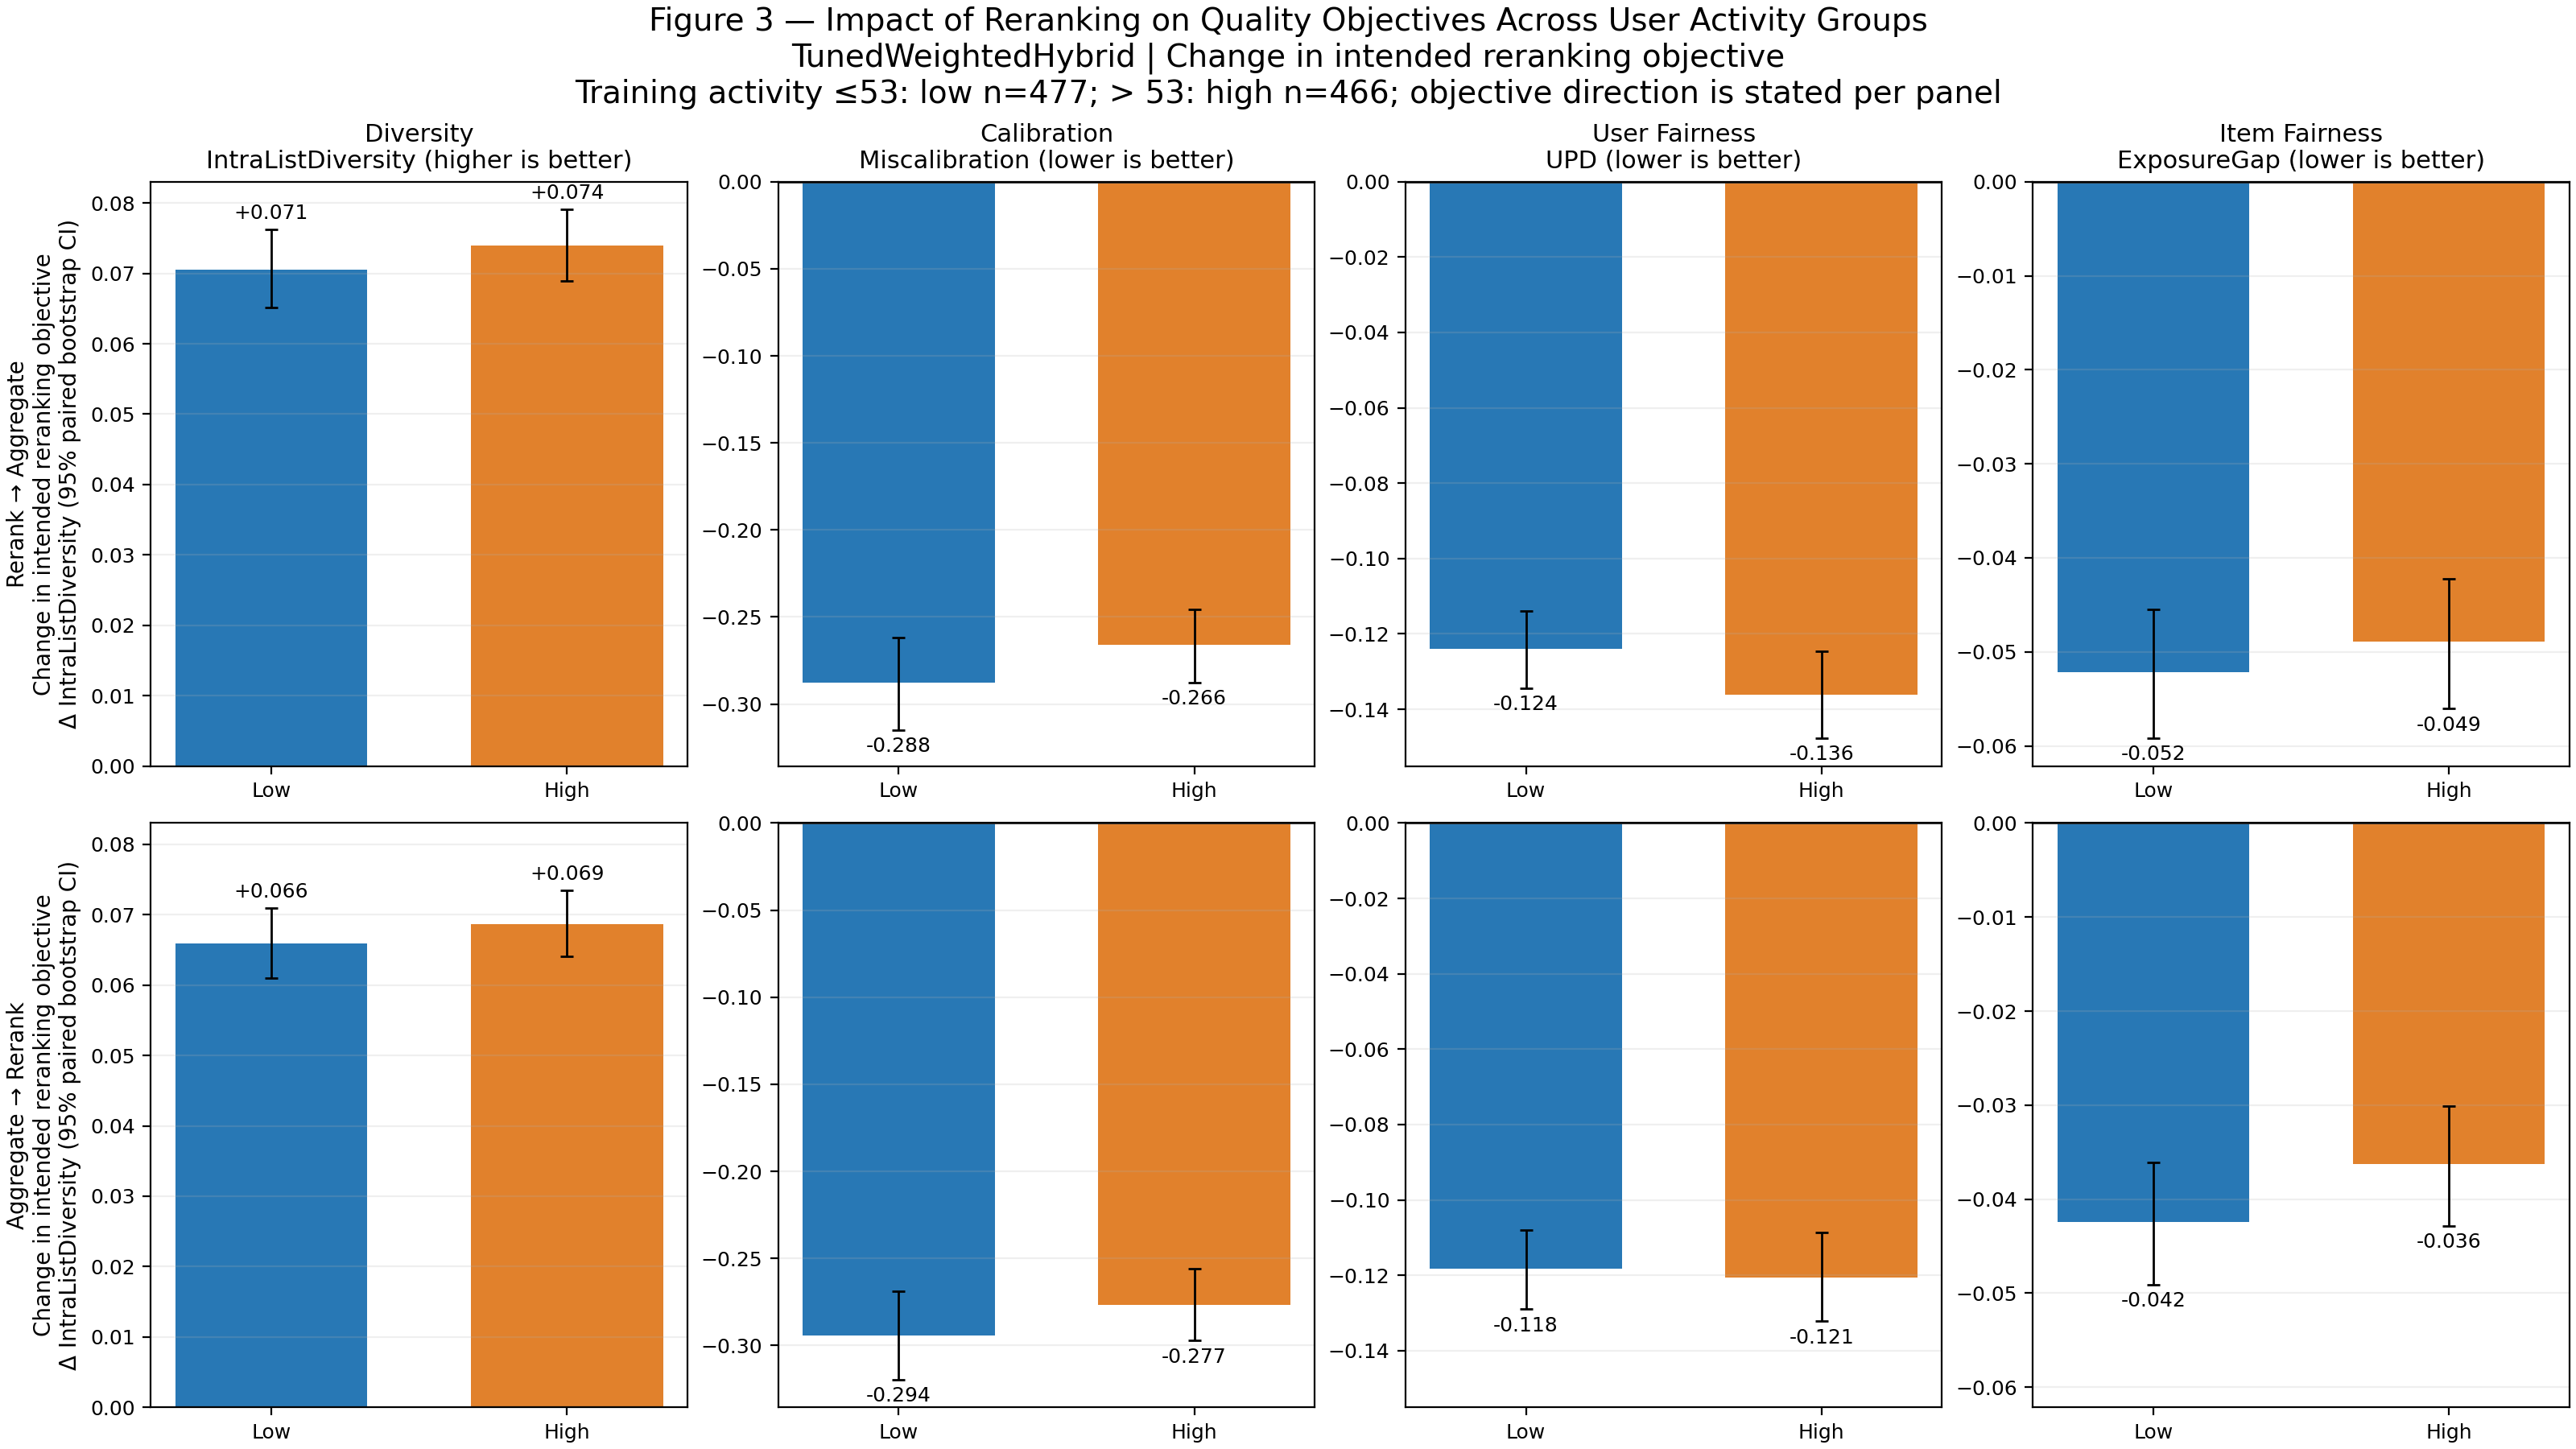
\includegraphics[
  width=0.8\linewidth,
  height=0.38\textheight,
  keepaspectratio
]{fig/fig_task3.4_user.png}
\caption{Reranking effects across low- and high-activity
users for both pipelines. Error bars show paired 95\%
user-bootstrap confidence intervals.}
\label{fig:task34_user}
\end{figure}

\paragraph{Discussion.}
Numerical examples refer to Aggregate $\rightarrow$ Rerank.
Calibration reduces miscalibration from .675 to .381 for
low-activity users and .672 to .395 for high-activity users.
User fairness reduces UPD by approximately .12 in both
groups, but its accuracy costs differ: nDCG changes by
-.0078 for low-activity users and +.0004 for high-activity
users. Their paired 95\% intervals are
$[-.0127,-.0032]$ and $[-.0034,+.0043]$, respectively.
Item fairness similarly changes nDCG by -.0041 and +.0027.
Thus comparable objective improvements can conceal
unequal accuracy costs; these observations are not a
formal test of between-group effects.

Item fairness increases discounted tail exposure from
0.8\% to 4.8\% and tail micro recall from .0080 to .0277,
so redistribution retrieves additional relevant tail
films. Nevertheless, exposure remains far below the
tail's 80\% catalogue share. Reranking improves the
targeted proxies without establishing complete fairness.
The candidate pool bounds possible changes, but its
contribution to the remaining exposure gap was not
separately tested. Confidence intervals describe
test-user sampling uncertainty within one split.
\clearpage
\appendix

\renewcommand{\thetable}{\thesection.\arabic{table}}
\renewcommand{\thefigure}{\thesection.\arabic{figure}}

\section{Supplementary reranking evidence}
\label{app:task3}

\setcounter{table}{0}
\setcounter{figure}{0}

\subsection{Reranking effects across base models}

Table~\ref{tab:appendix-reranking} supplements Task~3.2
with results for EASE, FeatureCombination and Pop.
Each change is measured against the corresponding
model's unreranked baseline from the same experiment.
All strengths were selected on validation before testing.

\begin{table}[htbp]
\centering
\begingroup
\setlength{\tabcolsep}{3pt}
\begin{tabular}{llrrrrrr}
\toprule
Model & Reranker & $\lambda$
& $\Delta$nDCG & $\Delta$ILD & $\Delta$KL
& $\Delta$UPD & $\Delta$Cov. \\
\midrule
EASE & Diversity & .25
& $-.0060$ & $+.0691$ & $-.1371$ & $+.0015$ & $-.0125$ \\
& Calibration & .10
& $-.0020$ & $+.0343$ & $-.2993$ & $-.0021$ & $+.0036$ \\
& User fairness & .25
& $-.0050$ & $-.0086$ & $+.0057$ & $-.1298$ & $+.0898$ \\
& Item fairness & .25
& $-.0001$ & $-.0060$ & $+.0016$ & $-.0480$ & $+.0571$ \\
\midrule
FeatComb & Diversity & .25
& $-.0030$ & $+.1094$ & $-.1950$ & $+.0036$ & $-.0048$ \\
& Calibration & .10
& $-.0021$ & $+.0523$ & $-.3575$ & $+.0011$ & $+.0006$ \\
& User fairness & .25
& $-.0100$ & $-.0163$ & $+.0380$ & $-.1288$ & $+.0850$ \\
& Item fairness & .25
& $-.0079$ & $-.0114$ & $+.0226$ & $-.0630$ & $+.0660$ \\
\midrule
Pop & Diversity & .50
& $+.0055$ & $+.1145$ & $-.3744$ & $.0000$ & $+.0089$ \\
& Calibration & .50
& $+.0032$ & $+.0526$ & $-.7241$ & $.0000$ & $+.0452$ \\
& User fairness & .50
& $-.0028$ & $-.0016$ & $+.0004$ & $-.0120$ & $+.0036$ \\
& Item fairness & .75
& $-.0060$ & $-.0012$ & $+.0004$ & $-.0106$ & $+.0065$ \\
\bottomrule
\end{tabular}
\endgroup
\caption{Held-out test changes at $K=10$ on the
seed-2020 split. Positive changes are desirable for
nDCG, ILD and coverage; negative changes are desirable
for genre miscalibration (KL) and popularity-preference
deviation (UPD). Coverage is a catalogue fraction.
Changes are absolute metric differences, rounded
to four decimal places. FeatComb denotes
FeatureCombination.}
\label{tab:appendix-reranking}
\end{table}

% Keep this reference only once in the report.
% Remove this paragraph if it already appears in your bibliography.
\paragraph{Reference.}
H.~Steck. Calibrated recommendations.
In \emph{Proceedings of RecSys}, 2018.

\clearpage
\subsection{Validation trade-offs for hybrid reranking}
\label{app:reranking-tradeoffs}

Figure~\ref{fig:appendix-validation-tradeoffs}
supplements Task~3.3 by showing the tested strengths,
including settings rejected by the accuracy constraint.

\begin{figure}[htbp]
\centering
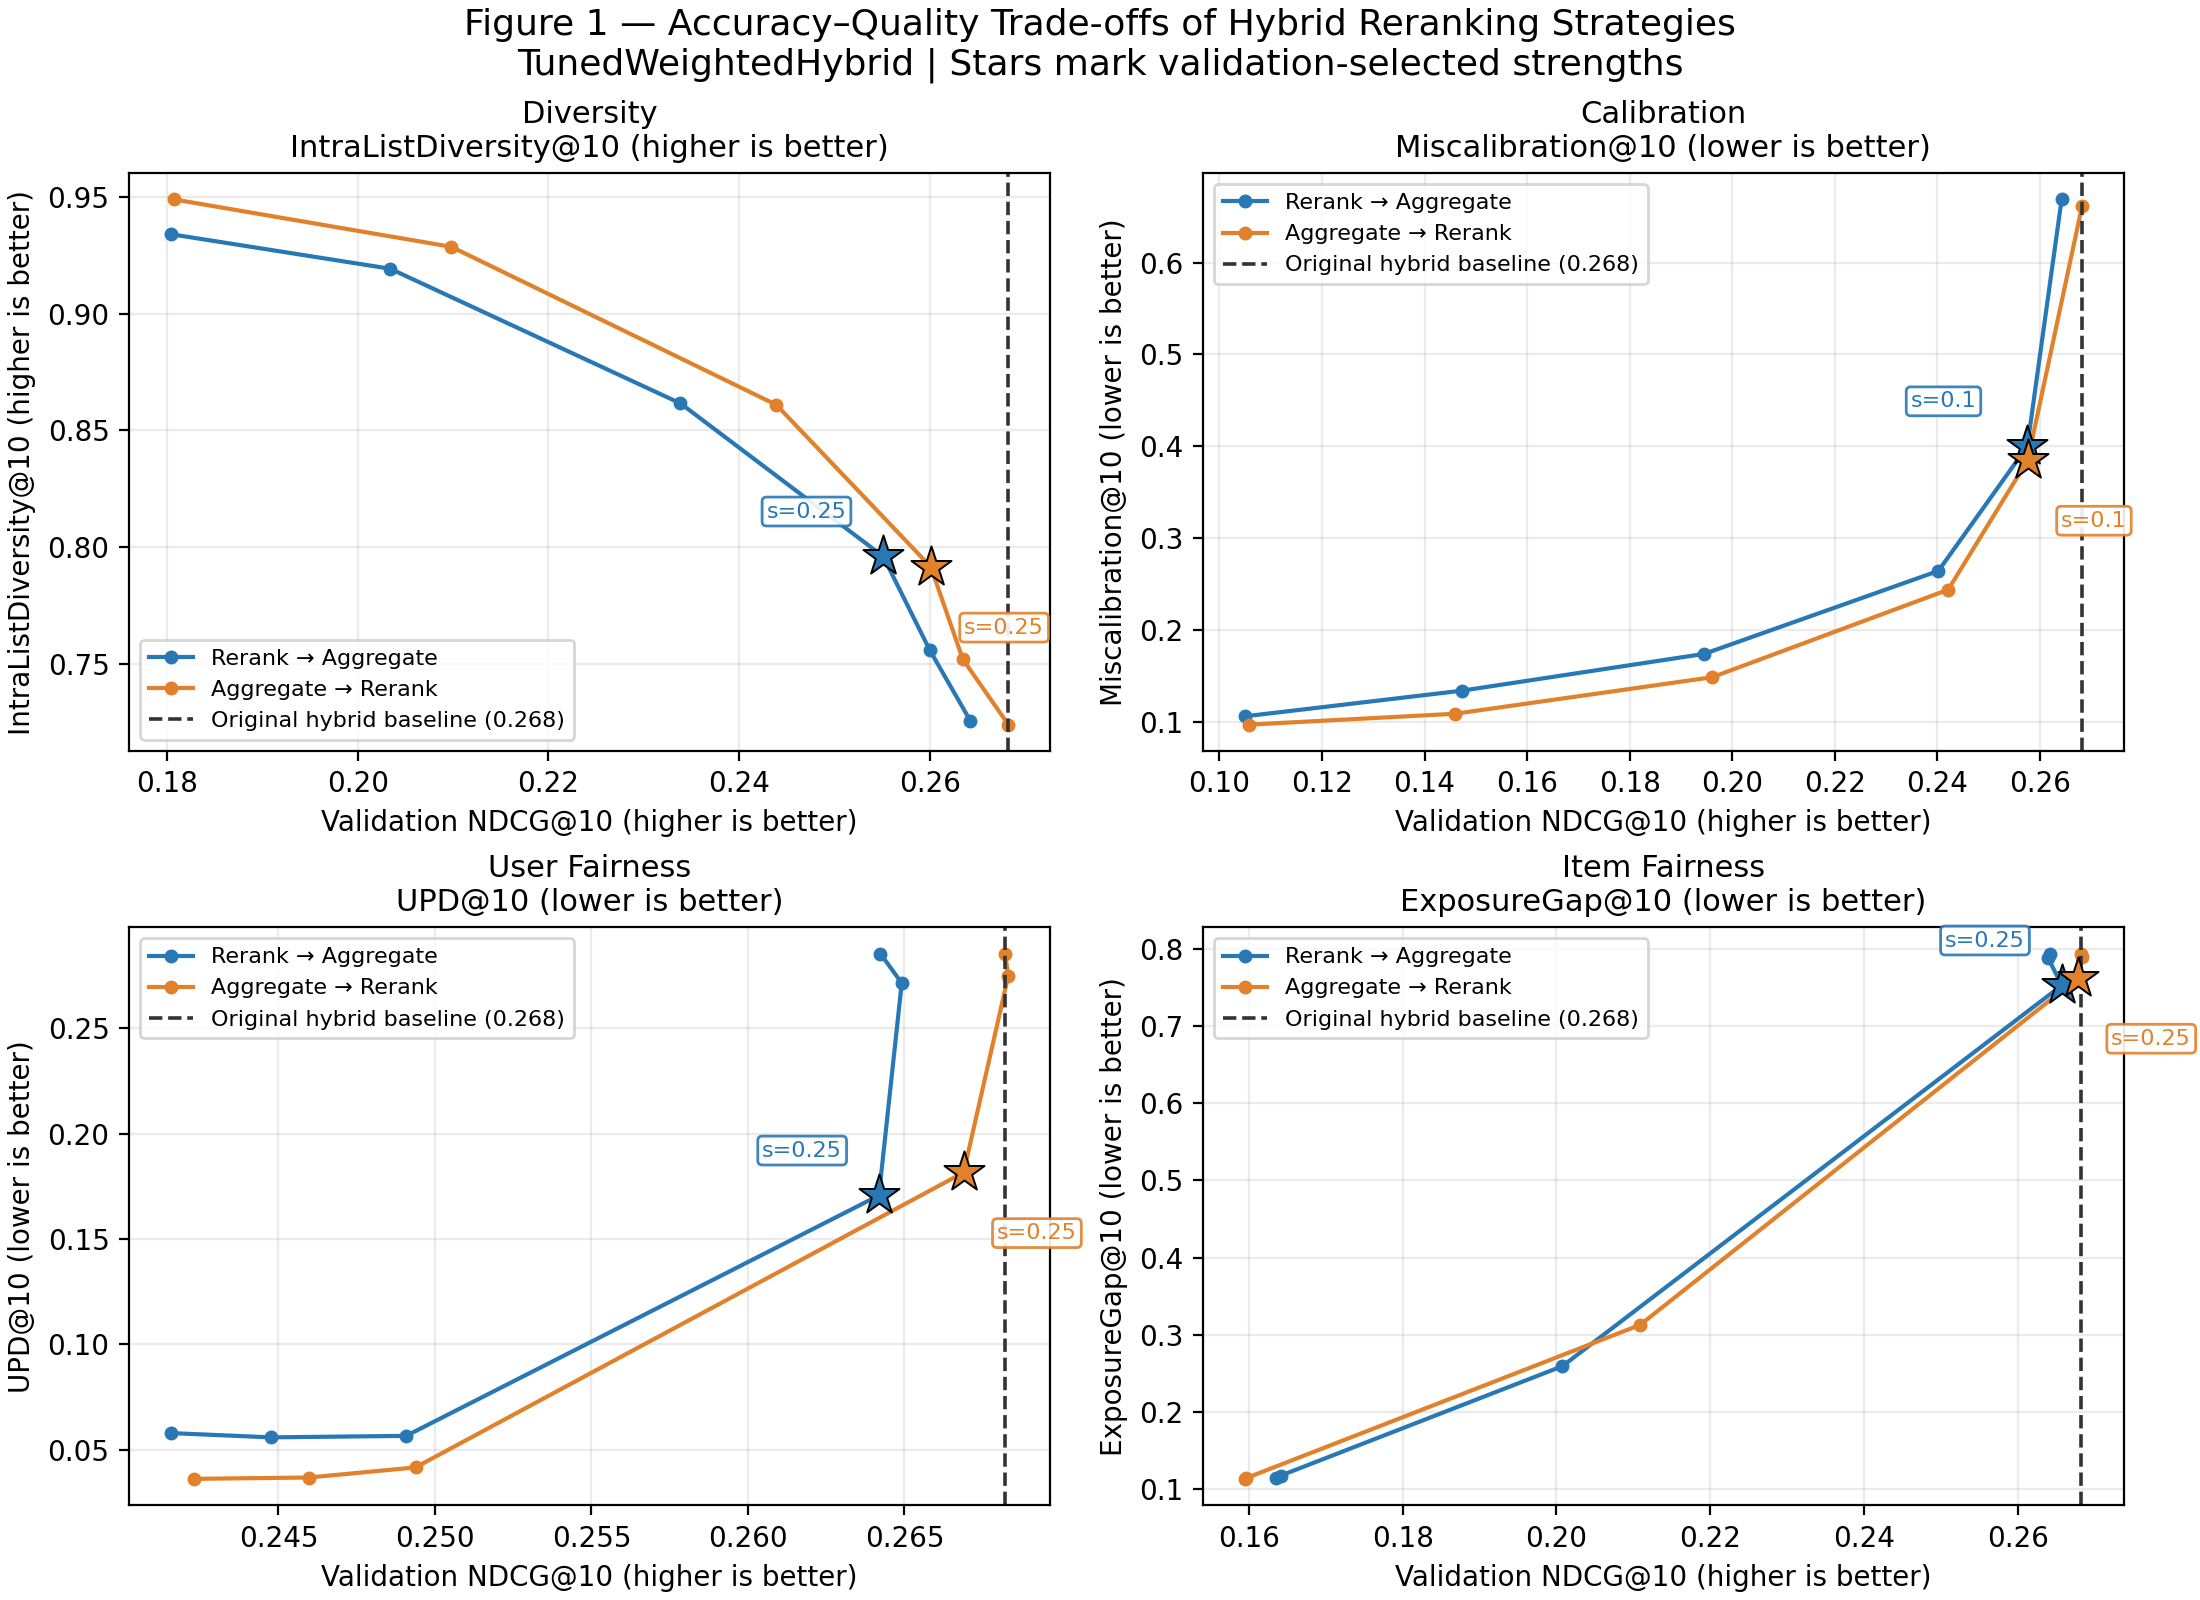
\includegraphics[
    width=\linewidth,
    height=0.68\textheight,
    keepaspectratio
]{fig/fig_task3_val.png}
\caption{Validation trade-offs for TunedWeightedHybrid.
Stars mark the selected strengths. Selection maximises
the targeted objective subject to at most 5\% relative
nDCG@10 loss against each pipeline's own zero-strength
baseline. The dashed line shows the original unreranked
score-hybrid baseline; it is not a separate depiction
of both pipelines' selection thresholds.
Component-first aggregation uses rank scores, whereas
aggregate-first aggregation uses normalised prediction
scores, so these curves compare complete pipeline designs.
Validation results are development evidence, not
independent estimates of generalisation.}
\label{fig:appendix-validation-tradeoffs}
\end{figure}

\clearpage
\subsection{Changes in item-group exposure}
\label{app:item-exposure}

Figure~\ref{fig:task34_item} supplements Task~3.4.
Head items are the 337 most popular training items;
the remaining 1,345 items form the tail.
The same groups and validation-selected strengths
are used for both pipelines.

\begin{figure}[htbp]
\centering
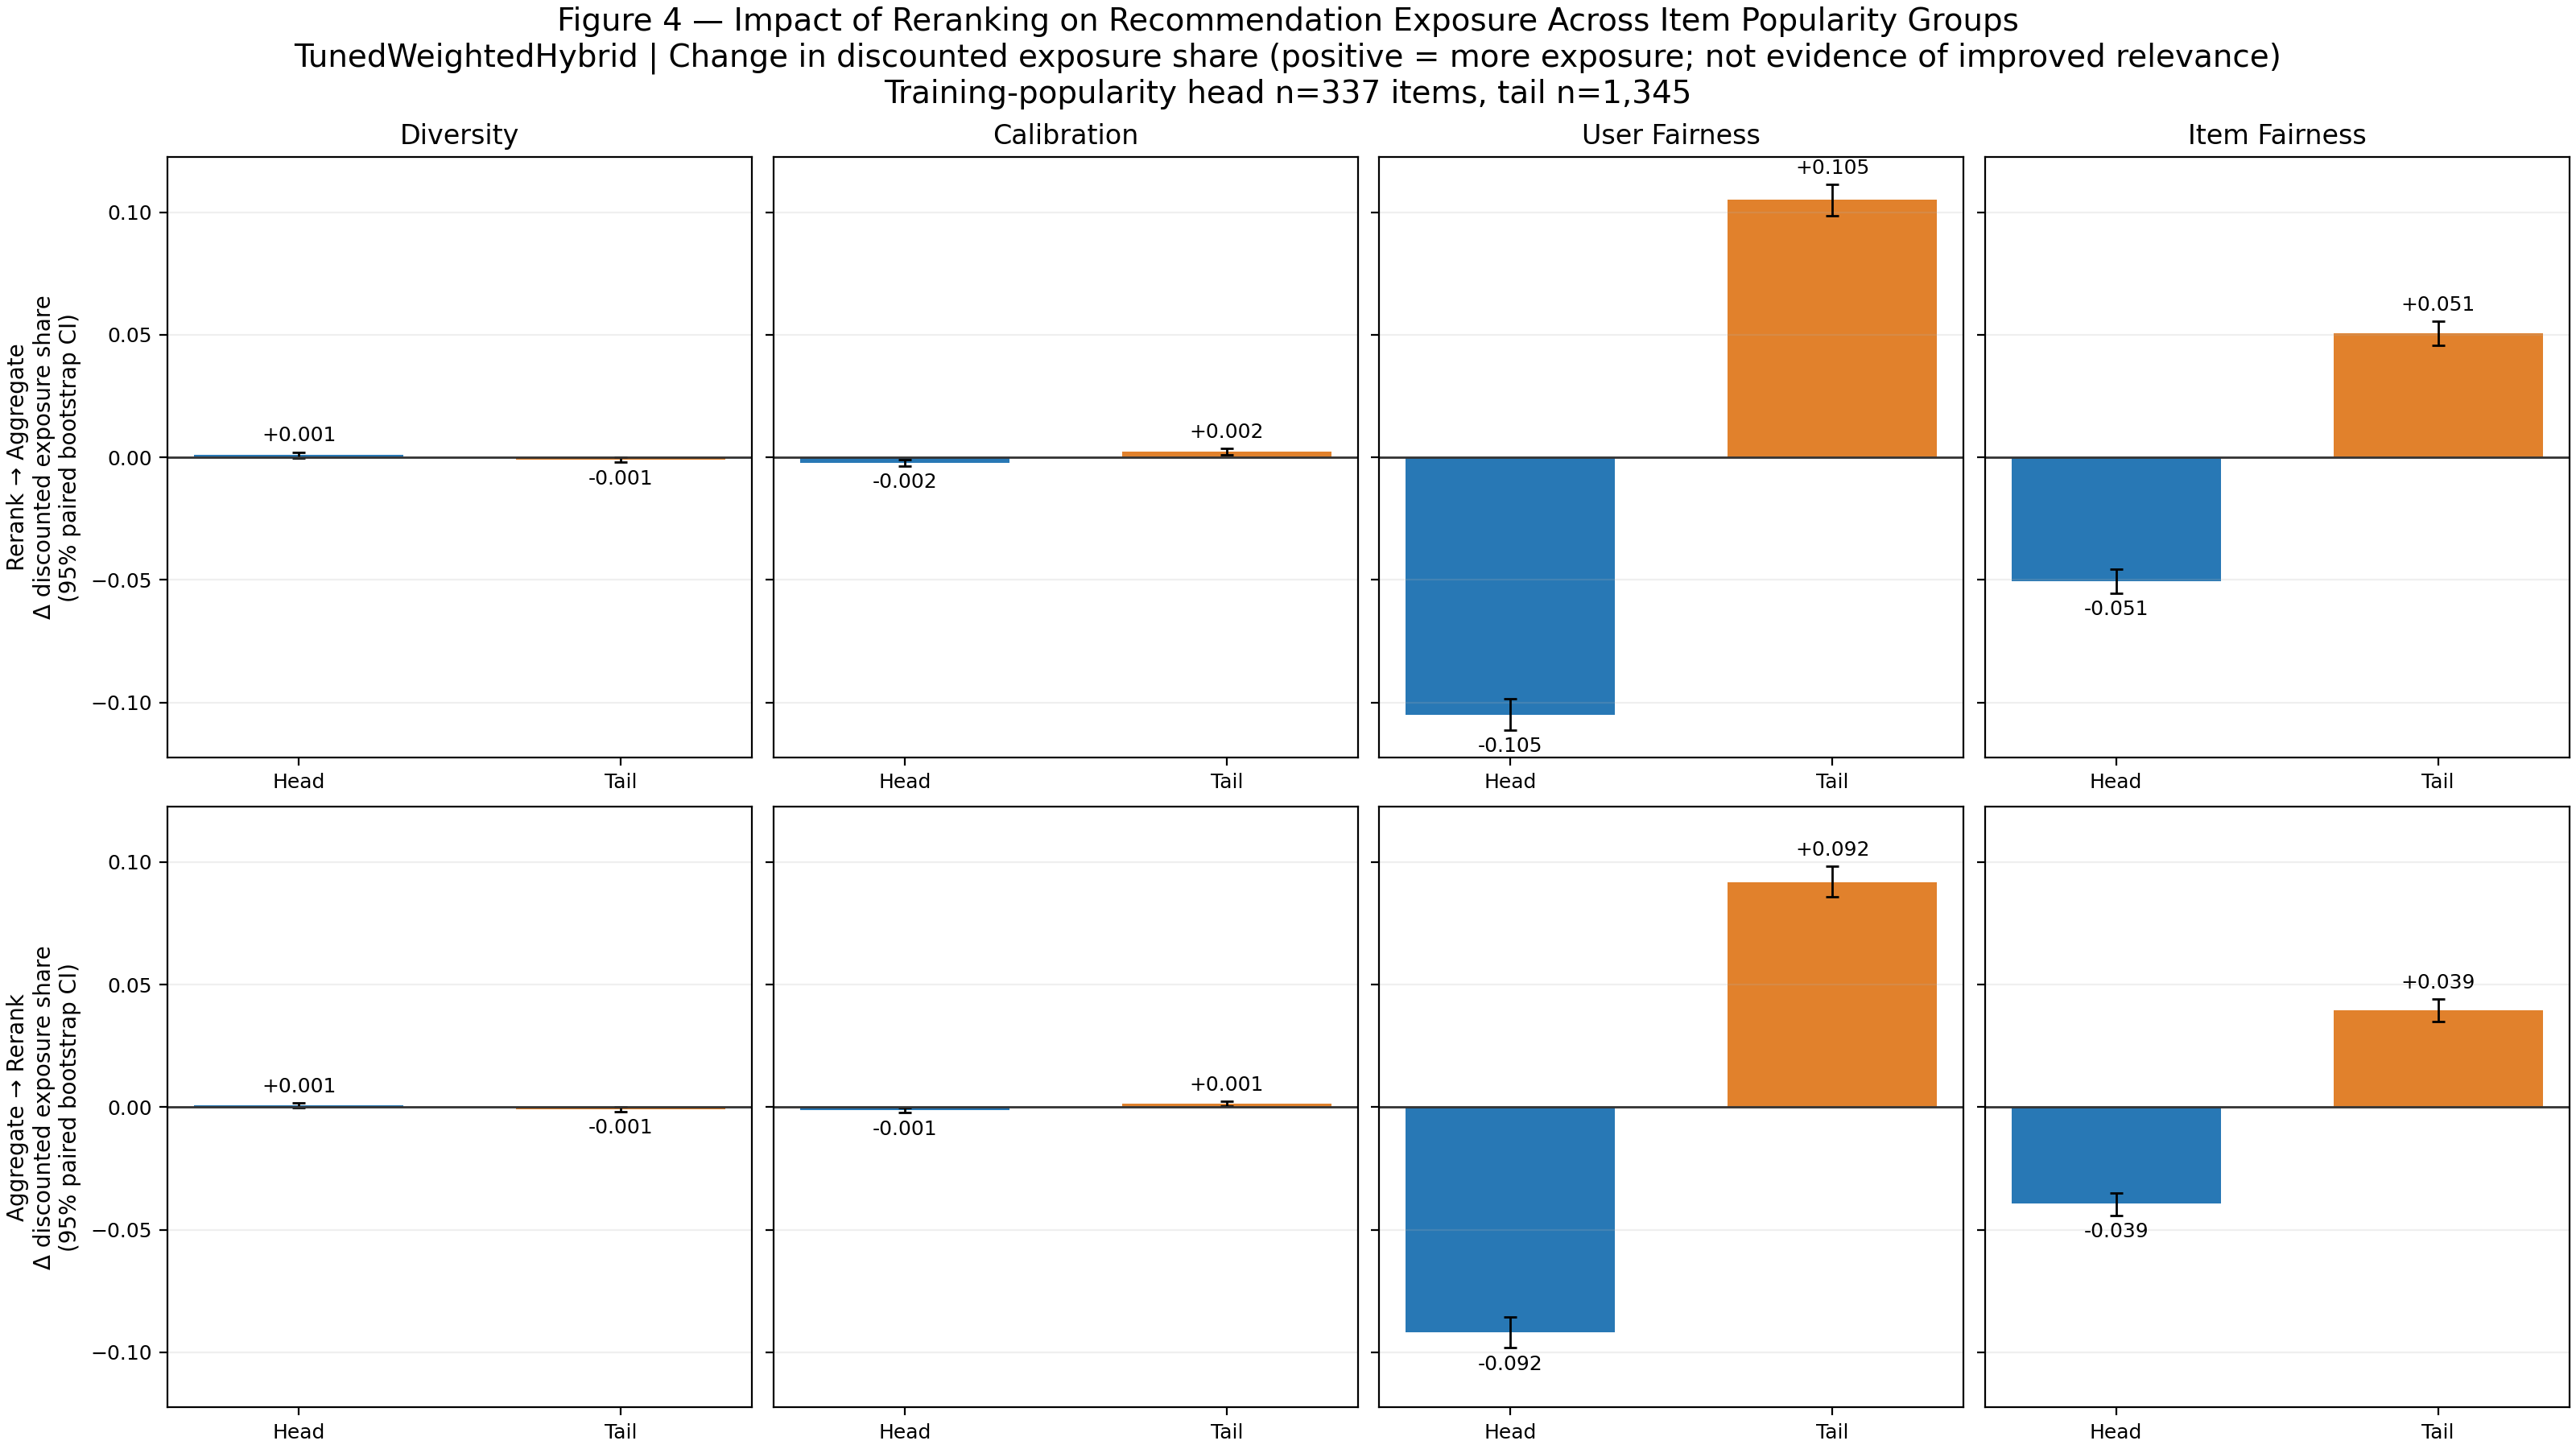
\includegraphics[
    width=\linewidth,
    height=0.62\textheight,
    keepaspectratio
]{fig/fig_task3.4_item.png}
\caption{Held-out changes in rank-discounted exposure
share relative to the original unreranked score-hybrid
ranking. The upper row shows component-first reranking
and rank aggregation; the lower row shows score
aggregation followed by reranking. Error bars are
paired 95\% bootstrap confidence intervals from
4,000 user resamples. Changes are exposure fractions:
$+.05$ represents five percentage points.
Head and tail changes sum to zero.
Exposure redistribution does not itself establish
improved relevance or equal accuracy across user groups.}
\label{fig:task34_item}
\end{figure}

\end{document}
